
\subsection{2.7. Диаграммы МО многоатомных молекул для описания химических и магнитных свойств. Потенциал ионизации молекулы.} 

\par\bigskip
	
С помощью диаграмм МО можно определить, является ли
молекула или ион парамагнитной или диамагнитной, её порядок и
кратность связи а также то, чем оно является: кислотой или
основанием Льюиса.

\par\smallskip	


Чтобы построить диаграмму МО для многоатомной молекулы,
лучше использовать аппарат симметрии. Согласно такому подходу,
перекрываться будут орбитали одинаковой симметрии. Если у
какой-либо орбитали нет пары по симметрии, она выступит, как
несвязывающая.

\par\smallskip	


Рассмотрим, как строить диаграмму МО с помощью аппарата
симметрии на примере молекулы воды.

\par\smallskip	

Для начала надо определить точечную группу симметрии - $C_{2v}$.
Затем надо определить оси в молекуле. Ось $z$ выбирают так, чтобы
она совпадала с осью высшего порядка (если она одна).

\begin{figure}[H]
	\centering
	{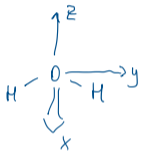
\includegraphics[scale=1.5]{19.png}}
\end{figure}	


Далее выписываются орбитали всех атомов (все или только
интересующие) в столбик, а в строчку - все операции симметрии.
Чтобы не забыть про какую-либо из них, надо воспользоваться
таблицей характеров. 

\begin{figure}[H]
	\centering
	{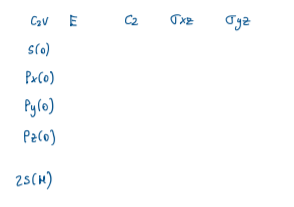
\includegraphics[scale=1.5]{20.png}}
\end{figure}


На пересечении каждого столбца и каждой клетки стоит характер
матрицы для данной операции - сумма элементов, находящихся на
главной диагонали. В таблице характеров для центрального атома
уже расписаны все характеры для центрального атома. Чтобы
понять, к какой орбитали это относится, надо посмотреть во второй
гиперстолбец таблицы - там можно найти обозначения $x, y, z, xy,
yz, xz, x^2-y^2, z^2$.

\begin{figure}[H]
	\centering
	{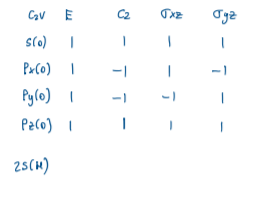
\includegraphics[scale=1.5]{21.png}}
\end{figure}


Для нецентральных атомов надо определить характеры матриц
самостоятельно. Если в результате применения данной операции
симметрии орбиталь остаётся на месте и не меняет знак, то ей
соответствует значение 1, если меняет знак, то -1. Если орбиталь
изменяет свое местоположение, то значение 0. Также могут
использоваться матрицы поворота:

\begin{figure}[H]
	\centering
	{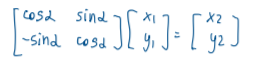
\includegraphics[scale=1.5]{22.png}}
\end{figure}



В зависимости от того, сколько орбиталей рассматривалось вместе,
надо сложить столько же вышеназванных значений.

\begin{figure}[H]
	\centering
	{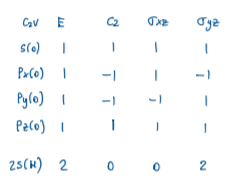
\includegraphics[scale=1.5]{23.png}}
\end{figure}

Каждая строчка для центрального атома представляет собой так
называемое неприводимое представление. Для нецентральных
атомов - приводимое. Оно раскладывается на линейную
комбинацию неприводимых представлений единственным образом.
Это можно или подобрать вручную, или воспользоваться формулой
приведения. Неприводимые представления определяются с
помощью таблицы характеров.

\begin{figure}[H]
	\centering
	{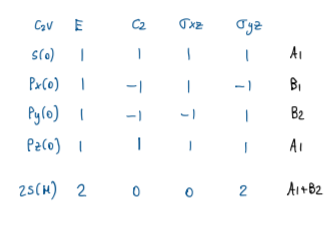
\includegraphics[scale=1.5]{24.png}}
\end{figure}


Теперь строится диаграмма МО. Как уже было сказано, орбитали, у
которых нет пары по симметрии, выступят, как несвязывающие.
Благодаря рисунку, можно представлять, какие орбитали будут
перекрываться лучше, а какие - хуже.

\begin{figure}[H]
	\centering
	{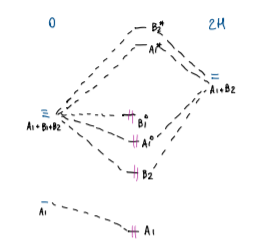
\includegraphics[scale=1.5]{27.png}}
\end{figure}

Орбитали заполняют электронами, начиная с самой нижней. Теперь
можно определить некоторые свойства. Поскольку нет
неспаренных электронов, молекула диамагнитна. Порядок связи
равен двум, а кратность единице (поскольку два заместителя у
центрального атома). Видно, что если система присоединит
электронную пару, то нарушится устойчивая восьмиэлектронная
система, электронов будет слишком много. Восьмиэлектронная
система нарушится и при отдаче электронной пары, более того,
поскольку ЭП на ВЗМО находится у атома кислорода, у него тяжело
отобрать ЭП, потому что он высокоэлектроотрицательный элемент.
Однако ЭП находится на несвязывающей орбитали, следовательно,
при отдаче не изменится порядок и кратность связи. Итого, это
плохое основание Льиса (плохой донор ЭП).

\par\smallskip	


Итак, если у молекулы есть неспаренные электроны, она
парамагнитна, если нет, то диамагнитна. Кратность и порядок связи
считаются по формулам:

\begin{figure}[H]
	\centering
	{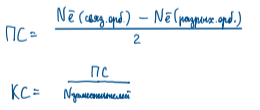
\includegraphics[scale=1.5]{25.png}}
\end{figure}

Молекула будет кислотой Льюиса, если её LUMO - несвязывающая
орбиталь, особенно, если приведёт к образованию 8-электронной
системы (например, для BH3). Возможно акцептирование ЭП и на
разрыхляющие орбитали, но тогда КС должна оставаться не меньше
единицы.

\par\smallskip	

Молекула будет основанием Льюиса, если она способна отдавать
ЭП (особенно, когда образуется 8-электронная система из 10-
электронной, например, СО).

	

\begin{center}
\textbf{Потенциал ионизации молекулы.}
\end{center}


Потенциал ионизации - это работа, которая требуется, чтобы
оторвать один электрон с высшего занятого электронами уровня.
Так, первый потенциал ионизации соответствует отрыву электрона
с HOMO. Таким образом, потенциал ионизации молекулы равен
взятой с обратным знаком одноэлектронной энергии
соответствующей МО.

\par\smallskip	

Например, для молекулы метана два первых потенциала
ионизации (можно оторвать электрон с А1 и с Т2, для Т2
потребуется больше энергии), а в молекуле воды их четыре (по
увеличению требуемой энергии - В1(нсв), А1(нсв), В2, А1).
	
	
\begin{figure}[H]
	\centering
	{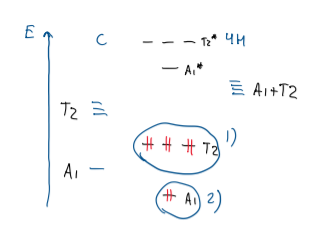
\includegraphics[scale=1.5]{26.png}}
\end{figure}	
	
	
\par\bigskip
\par\bigskip
